\documentclass{include/thesisclass}
\usepackage{tabularx}
\usepackage{changepage}
\usepackage{subfig}
\usepackage{float}
\usepackage[outputdir=out]{minted}
\usemintedstyle{pastie}
% \usepackage[printonlyused,withpage]{acronym}
% \usepackage[draft]{showlabels}
% \showlabels{cite}
% \showlabels{gls}
% \showlabels{todo}

\usepackage{csquotes}
\usepackage[acronym,toc]{glossaries}
\setacronymstyle{long-short}
\makeglossaries
\newacronym{LM}{LM}{Language Model}
\newacronym{LLM}{LLM}{Large Language Model}
\newacronym{NER}{NER}{Named Entity Recognition}
\newacronym{ER}{ER}{Entity Recognition}
\newacronym{MOF}{MOF}{Metal Organic Framework}


\newacronym{TF-IDF}{TF-IDF}{Term Frequency - Inverse Document Frequency}
\newacronym{BM25}{BM25}{\todo{explain bm25}}
\newacronym{BERT}{BERT}{Bidirectional Encoder Representation from Transformers}
\newacronym{SOTA}{SOTA}{State of the Art}
\newacronym{NLP}{NLP}{Natural Language Processing}





\newglossaryentry{GPT2}{
    name=GPT2,
    description={The second generation \textbf{G}enerative \textbf{P}retrained \textbf{T}ransformer \gls{LM} from \gls{OpenAI} \cite{radford_language_2019}.}
}

\newglossaryentry{GPT3}{
    name=GPT3,
    description={The third generation \textbf{G}enerative \textbf{P}retrained \textbf{T}ransformer \gls{LM} from \gls{OpenAI} \cite{brown_language_2020}.}
}

\newglossaryentry{GPT4}{
    name=GPT4,
    description={The fourth generation \textbf{G}enerative \textbf{P}retrained \textbf{T}ransformer \gls{LM} from \gls{OpenAI} \cite{openai_gpt4_2023}. Currently their most capable model.}
}

\newglossaryentry{bloom}{
    name=BLOOM,
    description={BigScience Large Open-science Open-access Multilingual Language Model, a 176 billion parameter open-source \gls{LLM} trained on \gls{Google} infrastructure in a concerted effort also including \gls{hf} and other organizations}
}


\newglossaryentry{opt}{
    name=OPT,
    description={Open Pretrained Transformer, a 178 billion parameter open-source \gls{LM} from \gls{Meta} research}
}

\newglossaryentry{Meta}{
    name=Meta,
    description={Previously known as Facebook, Meta regularly open-sources \gls{SOTA} \glspl{LLM}
    }
}

\newglossaryentry{OpenAI}{
    name=OpenAI,
    description={American company at the frontier of scaling deep learning architectures. Models that pushed boundaries include \glspl{LM} such as \gls{GPT2}, \gls{GPT3} and \gls{GPT4} as well as image generation models}
}

\newglossaryentry{Google}{
    name=Google,
    description={Search Engine giant}
}

\newglossaryentry{hf}{
    name=HuggingFace,
    description={American deep learning ecosystem Startup}
}


\interfootnotelinepenalty=10000

\newcommand{\vect}[1]{\boldsymbol{\bm{#1}}} % for package bm

\SelectLanguage{english}
% details on this thesis
\newcommand{\thesisauthor}{Felix Karg}
%\newcommand{\thesistopic}{Name des Themas auf Deutsch}

%\newcommand{\thesisentopic}{Extraction of structural information from powder X-ray diffraction patterns
%using neural network based on randomly generated crystals}
%\newcommand{\thesisentopic}{Analysis of Powder X-Ray Diffractograms
%Using Neural Networks Trained on an Infinite Stream of Synthetic Patterns}
%\newcommand{\thesisentopic}{Analysis of Powder X-Ray Diffractograms
%Using Neural Networks Trained on Continuously Generated Synthetic Patterns}
%\newcommand{\thesisentopic}{Analysis of Powder X-ray Diffractograms Using Neural Networks Based on
%Synthetic Patterns Generated During Training}
%\newcommand{\thesisentopic}{Analysis of Powder X-Ray Diffractograms
%Using Neural Networks Trained on Continuously Generated Synthetic Patterns}
\newcommand{\thesisentopic}{A Benchmark on Using Large Language Models for Zero-Shot Automated Data Extraction from Scientific Literature}

\newcommand{\thesisinstitute}{Institute of Theoretical Informatics}
\newcommand{\thesisreviewerone}{T.T.-Prof. Dr. Pascal Friederich}
\newcommand{\thesisreviewertwo}{Prof. Dr. Second Reviewer}
\newcommand{\thesisadvisorone}{Tobias Schlöder}
\newcommand{\thesistimestart}{2023-03-01} % on titlepage
\newcommand{\longdate}{2nd October 2023} % on signature lines
\newcommand{\thesistimeend}{2023-10-02} % on titlepage
\newcommand{\thesistimehandin}{2023-10-02} % on second page 'preamble'
\newcommand{\thesispagehead}{\thesisentopic} % page heading


% ----------------- referencing ----------------
\newcommand{\secref}[1]{Section~\ref{sec:#1}}
\renewcommand{\subref}[1]{Subsection~\ref{sub:#1}}
\newcommand{\chapref}[1]{Chapter~\ref{chap:#1}}
\renewcommand{\eqref}[1]{Equation~(\ref{eq:#1})}
\newcommand{\figref}[1]{Figure~\ref{fig:#1}}
\newcommand{\tabref}[1]{Table~\ref{tab:#1}}
\newcommand{\coderef}[1]{Code Example~\ref{code:#1}}
\newcommand{\outref}[1]{Output~\ref{out:#1}}

\newcounter{code}
\setcounter{code}{0}
\newenvironment{codeboxed}[2]{
    \begin{minipage}{\linewidth}\begin{center}\textbf{#1}\\\small #2\\[1ex]\begin{tabular}{|p{\textwidth}|}\hline}{
    \\\hline\end{tabular}\end{center}\end{minipage}}

\newcommand{\code}[3]{\refstepcounter{code}\label{code:#2}\begin{codeboxed}{Code Example \thecode}{#3}
        \inputminted[linenos,fontsize=\small]{Python}{code/#1}\end{codeboxed}}


\hypersetup
{
    pdfauthor={\thesisauthor},
    pdftitle={\thesisentopic},
    pdfkeywords={kit,informatics,master,thesis,\thesisauthor}
}

% Describe separation hints here:
\hyphenation
{
    über-nom-me-nen an-ge-ge-be-nen
}

\addbibresource{references.bib}


\begin{document}

% Always use the primary source of information (probably mostly relevant in introduction)
% Referencing whole paragraph after full stop is fine (Harvard style).
% ~ is an unbreakable space.

% Punctuation for equations:
% - Use "equation" blocks
% - Use \,. to set a point after an equation.
% See: https://tex.stackexchange.com/questions/7542/for-formal-articles-should-a-displayed-equation-be-followed-by-a-punctuation-to

% Page numbers required for direct quotations.
% Can also be helpful for indirect quotations, for example to locate the source in a big book etc.
% For papers not necessary.

% Cite entire paragraph after final period: https://tu-dresden.de/bu/umwelt/geo/ifk/ressourcen/dateien/downloads/TUM-Citation-Guide.pdf?lang=de

\newcommand{\diameter}{20}
\newcommand{\xone}{-15}
\newcommand{\xtwo}{160}
\newcommand{\yone}{15}
\newcommand{\ytwo}{-253}

\fancypagestyle{alim}{\fancyhf{}\renewcommand{\headrulewidth}{0pt}
	\fancyfoot[R]{\footnotesize{\textbf{www.kit.edu}}}
	\fancyfoot[L]{\footnotesize{KIT – The Research University in the Helmholtz Association}}
}

\begin{titlepage}

	\thispagestyle{alim}

	\noindent
	% KIT image and sign for faculty of physics

	\noindent\begin{minipage}{0.25\textwidth}% adapt widths of minipages to your needs
		
\includegraphics[width=1\textwidth]{include/kitlogo.pdf}
	\end{minipage}
	\hfill
	\begin{minipage}{0.25\textwidth}\raggedleft
		
\includegraphics[width=1\textwidth]{include/AiMat_logo_purple.png}
	\end{minipage}

    \centering

    % thesis topic (en and ge)
	\vspace*{4.0cm}

	\large\par\noindent\rule{\textwidth}{1.2pt}

	\Huge \thesisentopic

	\large\par\noindent\rule{\textwidth}{1.2pt}

    % author name and institute
    \vspace*{2cm}
    \Large Master thesis\\by\\
    \vspace*{1cm}
    \huge\thesisauthor\\
    \vspace*{1cm}
    \Large \thesisinstitute

    % examiners (Referenten)
    \vspace*{4cm}
    \large
    \begin{center}
        \begin{tabular}[ht]{l c l}
        \iflanguage{english}{Reviewer}{Referent}: 
            & \hfill & \thesisreviewerone\\
        \iflanguage{english}{Second Reviewer}{Korreferent}: 
			& \hfill & \thesisreviewertwo\\
        \iflanguage{english}{Advisor}{Betreuender Mitarbeiter}: 
            & \hfill & \thesisadvisorone\\ \\
        % uncomment if you want to provide info on more than one advisor
        %\iflanguage{english}{Second Advisor}{Zweiter betreuender Mitarbeiter}: 
        %    & \hfill & \thesisadvisortwo\\
		\large{Begin:}
			& \hfill & \large{\thesistimestart}\\
			\large{Submission:}
            & \hfill & \large{\thesistimeend}\\
        \end{tabular}
    \end{center}

\end{titlepage}

\chapter*{Declaration of Authorship}

Find the appropriate and up-to-date text in your Studienordnung and copy it here.\\

\vspace{1cm}

\noindent Karlsruhe, Month dd, yyyy \hfill \parbox[t]{.5\linewidth}{\rule[-3pt]{\linewidth}{.4pt}\par\smallskip
    \centering Your name}

\vfill

Approved as examination copy:\\

\vspace{1cm}

\noindent Karlsruhe, Month dd, yyyy \hfill \parbox[t]{.5\linewidth}{\rule[-3pt]{\linewidth}{.4pt}\par\smallskip
    \centering}

\renewcommand{\arraystretch}{1}

\cleardoublepage

\addchap{Abstract}\label{chap:abstract}
\pagenumbering{arabic}

% How to write an abstract
%  One or two sentences providing a basic
%  introduction to the field, comprehensible to
%  a scientist in any discipline.
A majority of materials science knowledge is contained in unstructered text scattered throughout the body of scientific literature, out of reach for increasingly capable but data-starved \acrlong{ML} models that are being used more and more at every step of the materials creation process.
%  Two to three sentences of more detailed
%  background, comprehensible to scientists
%  in related disciplines.
Thus, the extraction of such information from unstructured scientific literature and conversion to machine-readable formats has become a challenge of \acrlong{NLP}.
Recently, \acrlongpl{LLM} have gained prominence for their general capabilities across \acrlong{NLP} tasks, including \acrlong{NER}.
%  One sentence clearly stating the general
%  problem being addressed by this particular
%  study.
%However, such information is often not accessible in a machine-readable format.
%  One sentence summarizing the main result
%  (with the words “here we show” or their
%  equivalent).
This work demonstrates that automated information extraction from materials science literature is possible with high accuracy using models of only 13 billion parameters and without fine-tuning.
%  Two or three sentences explaining what the
%  main result reveals in direct comparison to
%  what was thought to be the case previously,
%  or how the main result adds to previous
%  knowledge.
In fact, 13 billion parameter sized variants from both \model{llama} and \model{llama2} achieved an accuracy of 95 to 98\% for the extraction of temperature and time information from unstructured text.
Additionally, the 7 billion parameter sized \model{falcon} achieved an accuracy of 79\% on the extraction of solvent information from synthesis paragraphs on the creation of \acrlongpl{MOF}.
%Contrary to expectation, fine-tuning is harder than expected with few resources available.
%  One or two sentences to put the results
%  into a more general context.
The smaller size of these models, their open-access availability, and no necessity for additional fine-tuning enables the usage of most consumer hardware, making these capabilities far more accessible than previously expected.
%  Two or three sentences to provide a broader
%  perspective, readily comprehensible to a
%  scientist in any discipline.

% This means, that even for more sophisticated information extraction tasks fine-tuning might not be necessary, particularly with more generally capable models in the future.

\addchap{Zusammenfassung}
Deutsche Zusammenfassung hier. \todo{write zusammenfassung}


\cleardoublepage
% \pagenumbering{arabic}
% other page numbering styles:
% - arabic: use Arabic numerals (1, 2, 3, ...)
% - alph: use lowercase letters (a, b, c, ...)
% - Alph: use uppercase letters (A, B, C, ...)
% - roman: use lowercase roman numerals (i, ii, iii, ...)
% - Roman: use uppercase roman numerals (I, II, III, ...)




\chapter{Introduction}\label{chap:introduction}

% clear and concise:
%  Presentation of the topic and the background
Unstructured scientific literature contains a vast amount of materials science knowledge, and is the only place to get it.
However, this places it squarely out of reach for further processing, which makes it difficult or impossible to build on a large part of prior work.
%  Motivation of importance
\gls{ML} models are increasingly used in screening steps for materials discovery and property prediction \cite{saal_machine_2020, luo_mof_2022, choudhary_recent_2022}, among other steps.
% These models continue to get better, but often the biggest bottleneck is a lack of data.
In general, more high-quality data improves the output quality of \gls{ML} models considerably \cite{hoffmann_empirical_2022}.
%  Research gap, research question
Currently, the amount of data accessible to train such models is limited, \todo{@Tobias check} in particular from older or less known work.

Over the last year, \glspl{LLM} rose to public prominence since the launch of \gls{ChatGPT}.
Regardless of public perception, recent improvements across \gls{NLP} benchmarks are undeniable \cite{devlin_bert_2018, openai_gpt4_2023}.
In this work, \glspl{LLM} are used for information extraction of scientific text on synthesisizing \glspl{MOF}.

% Structure of the thesis
\draft{
Structure.
}
% Short summary of main results
\draft{
Results summary.
}

% \section{Motivation}
% Take for example the field of synthesizing Metal-Organic Frameworks (MOFs)
% \cite{zhou_introduction_2012}. While numerous detailed descriptions of
% synthesis procedures exist, they are not available in machine-readable formats,
% which prevents effective application of state-of-the-art techniques such as
% automated experimentation \cite{shi_automated_2021} or synthesis parameter prediction
% \cite{luo_mof_2022}. Thus, we intend to create a pipeline for deriving
% machine-readable information on MOF synthesis parameters from given questions
% on provided scientific articles.

% Motivation
% \begin{itemize}
%     \item vast amount of material science knowledge scattered across papers
%     \item often non-machine readable formats
%     \item makes it difficult or impossible to build on (all) prior work
%     \item results in tremendous duplicates and other unnecessary work
%     \item a lot of insights to be gained from such a database, as well as automated experimental design (and possibly execution)
% \end{itemize}


\section{Scientific Question}\label{sec:question}

The goals of this work are threefold:
\begin{enumerate}
    \item Demonstrate zero-shot automated information extraction from scientific literature using open-access \glspl{LLM}.
    \item Benchmark and compare the accuracy of currently available open-access \glspl{LLM} for the automated information extraction from scientific literature.
    \item Attempt fine-tuning of open-access \glspl{LLM} in order to increase accuracy.
\end{enumerate}

As part of this work, a highly flexible automated pipeline for the extraction of non-machine readable information in \gls{MOF} synthesis will be created.
The approach chosen in this work will be discussed in more detail \chapref{approach}, where the implementation is described in \secref{impl}, the models used in \secref{models}, and \secref{data} describes the source of data.


\newpage
collection of todos
\todo{find a first section for introduction chapter}

explain stuff somewhere
\todo{explain context length somewhere}
\todo{explain zero-shot somewhere}
\todo{explain causal and masked language models somewhere}

\chapter{Background}\label{chap:background}
\todo{write background}
Core meta points:
\begin{itemize}
    \item up to five pages background
    \item go from very general to very related to topic, end with questions to resolve
\end{itemize}

\section{General Work, Related}\label{sec:general}
\todo{think about it if I actually want to include this section}
ml models increasingly used in screening steps for materials discovery and property prediction
% “Machine learning in materials discovery: Confirmed predictions and their underlying approaches"
% “Recent advances and applications of deep learning methods in materials science"

\section{Related Work}\label{sec:related}
% \todo{write section}
\todo{related work is only entity recognition stuff}

\subsection{Rule-Based Entity Recognition}\label{sub:ER}
There have long been rule-based approaches for the recognition of individual
entities (e.g. Temperature). ChemTagger \cite{hawizy_chemicaltagger_2011}
and others \cite{beard_comparative_2019, huang_database_2020}
clearly demonstrated that simple rule-based systems can sometimes extract much
of the requested information. They can often
achieve high precision for simple, well-defined
tasks, but tend to be highly specialized and
are hard to adapt to differing circumstances.

\todo{establish ER and NER}



\todo{Notes from Jehona Talk, adapt accordingly}
\begin{itemize}
    \item Techniques like TF-IDF or BM25 ??
    \item 'it is called extractive because it extracts the answer from a agiven
        context, rather than generating a new answer'
    \item using haystack as llm framework
    \item using a document store and memorizing architecture? dense retrieval:
        'using dense embeddings rather than sparse ones'
    \item
\end{itemize}

\paragraph{BM25}

\gls{BM25} is a ranking function that ranks a set of documents based on the query terms appearing in each document, regardless of the inter-relationship between the query terms within a document (e.g., their relative proximity).

\paragraph{TF-IDF}
\gls{TF-IDF} is a handy algorithm that uses the frequency of words to determine how relevant those words are to a given document.

\section{Language Models for Data Extraction Tasks}
\todo{write lms for data extraction and then move it to background}
It was shown that fine-tuning \gls{BERT} for \gls{NER} tasks in materials science has good results \cite{zhao_finetuning_2021}.

\subsection{Using LLMs for Data Extraction}
Fine-tuning \gls{GPT3} with 100 manual and 500 partially augmented examples of data extraction
created one of the most sophisticated pipelines for information extraction \cite{dunn_structured_2022}.
Most of our work will be similar to theirs. However,
Chinchilla \cite{hoffmann_training_2022} and CoTR \cite{zhang_multimodal_2023}
demonstrated that while achieving impressive capability, such large models are
substantially overparametrized and undertrained. Additionally, while the
results are state-of-the-art, GPT3 is only accessible through the API of
OpenAI, a for-profit company. This considerably limits access to model
internals.

Our work differs from \cite{dunn_structured_2022} by addressing these two
caveats. Instead of GPT3, we use a similarly capable open-source model called
OPT \cite{zhang_opt_2022}. Self-hosting enables us to do deep introspection
necessary for state-of-the-art prompt engineering and gives us the required
freedom to attempt distillation \cite{sun_patient_2019}, which addresses
overparametrization. Distillation promises substantial model parameter
reduction with little loss in accuracy (50x parameter reduction while keeping
95\% accuracy), and has been confirmed to have similar compression characteristics
for other large language models.
\todo{rewrite section on LLMs}




\newpage
\section{Scientific Question}\label{sec:question}
\todo{expand scientific question}

how well can we automate the extraction of parameters from scientific data using \glspl{LLM} with zero-shot

The goal of this work is to benchmark the accuracy of open source \glspl{LLM} to
demonstrate automated extraction of unstructured text from scientific
literature and create an automated pipeline for the creation of a database with otherwise non-machine readable information on \gls{MOF} synthesis or similar tasks.

% By
% doing so, we create a training pipeline that can be a) self-hosted and b)
% adapted to other data extraction tasks. It may be provided as a service for
% other research groups.
%
% In this work, we will use OPT \cite{zhang_opt_2022} to empirically test how
% much accuracy can be improved via 1) fine-tuning and 2) prompt engineering.
% Additionally, we intend to 3) test how accuracy and compute requirements will be
% affected by reduction of model size via distillation \cite{sun_patient_2019}.
% A reduction in parameters would make it considerably less compute intensive to
% run the final model.

\chapter{Scientific Question}
The goal of this work is to use large language models to demonstrate automated
extraction of unstructured text from scientific literature for the creation of
a database with otherwise non-machine readable information on MOF synthesis. By
doing so, we create a training pipeline that can be a) self-hosted and b)
adapted to other data extraction tasks. It may be provided as a service for
other research groups.

In this work, we will use OPT \cite{zhang_opt_2022} to empirically test how
much accuracy can be improved via 1) fine-tuning and 2) prompt engineering.
Additionally, we intend to 3) test how accuracy and compute requirements will be
affected by reduction of model size via distillation \cite{sun_patient_2019}.
A reduction in parameters would make it considerably less compute intensive to
run the final model.

\todo{rewrite}


\section{Results}

\begin{frame}[c,fragile,allowframebreaks]{Accuracy Overview}
    \pause
    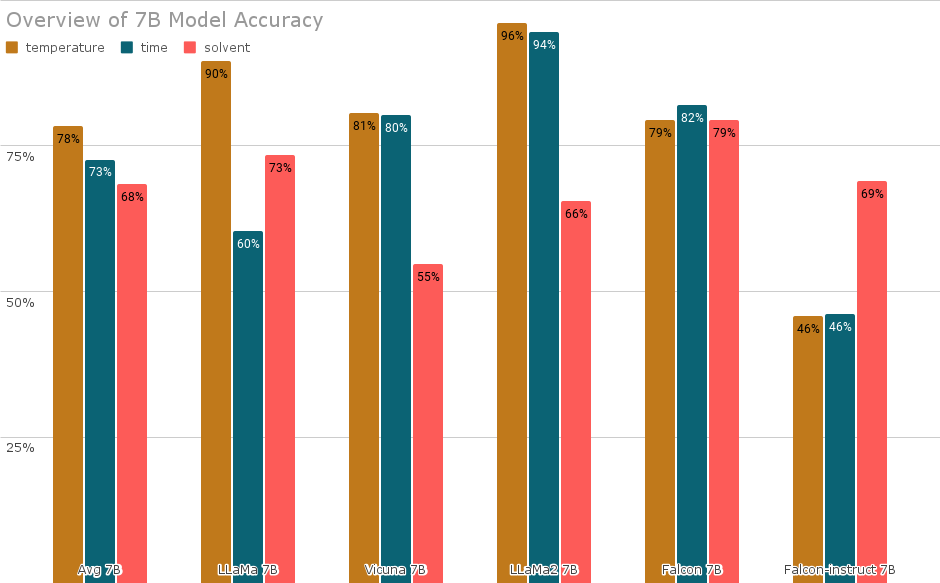
\includegraphics[height=0.7\textheight]{overview_7b_accuracy}
    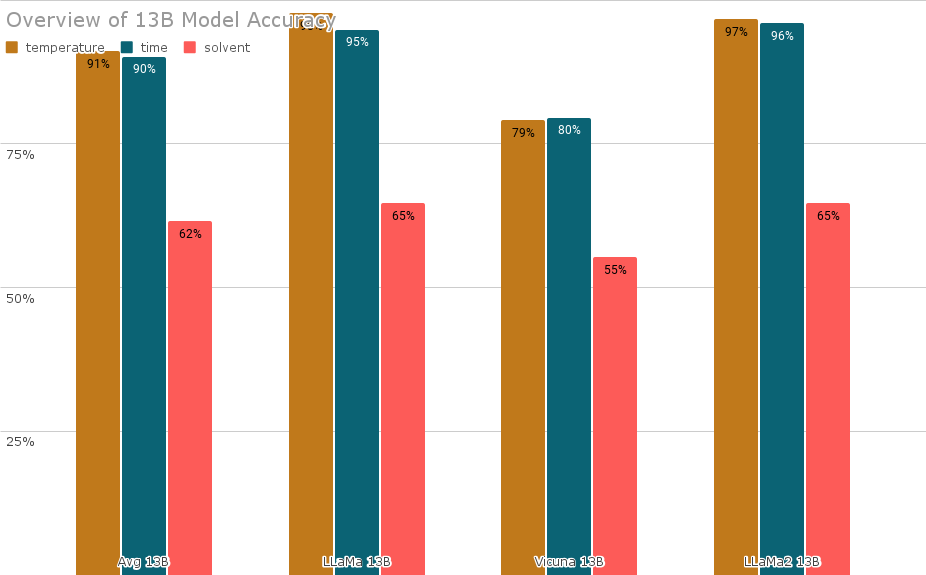
\includegraphics[height=0.7\textheight]{overview_13b_accuracy}
    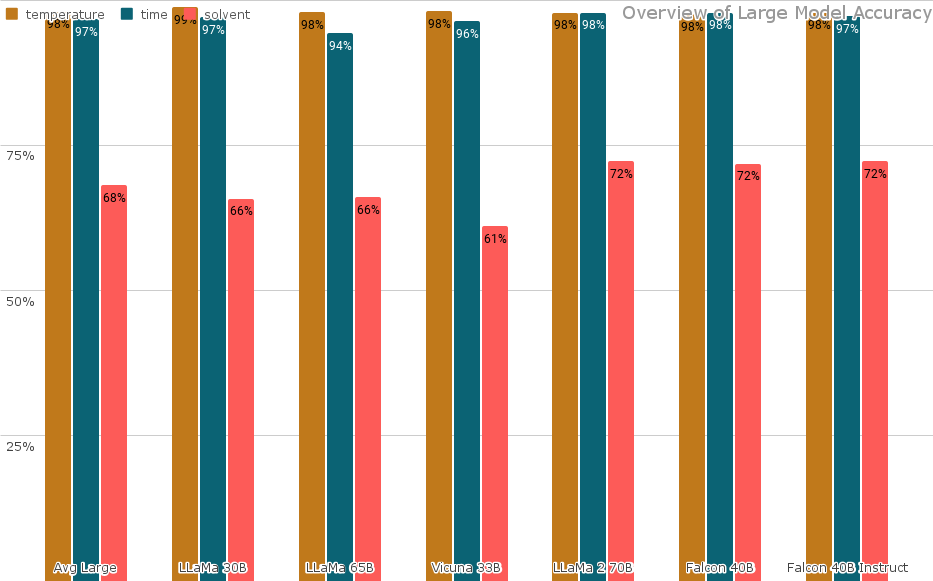
\includegraphics[height=0.7\textheight]{overview_large_accuracy}
\end{frame}



\begin{frame}<handout>[c]{Note on Interesting Outliers}
    \begin{columns}
        \column{0.3\textwidth}
    7B
    \begin{itemize}
        \item \gls{llama}-7B accuracy on \ttemp and \ttime vary substantially across models, but are mostly similar within one model
        \item \tsolv accuracy of \gls{vicuna} bad somehow
        \item Bad \ttemp and \ttime accuracy of \gls{falcon}-instruct
        \item Decent performance from \gls{llama2} overall
    \end{itemize}
        \column{0.3\textwidth}
        \large
        13B
        \begin{itemize}
            \item \gls{vicuna} still lagging behind, though while \gls{falcon} does not have a 13B variant, it should still be worse
            \item Accuracy on \tsolv seems to have gotten worse, on average and for individual models
        \end{itemize}
        \column{0.3\textwidth}
        \large
        30B+
        \begin{itemize}
            \item Average Accuracy very high
            \item \tsolv accuracy only 72\% though, that was higher in 7B models!
        \end{itemize}
    \end{columns}
\end{frame}

\subsection{Frequent Mistakes}

\begin{frame}[c,fragile,allowframebreaks]{Unit Confusion}
    \pause
    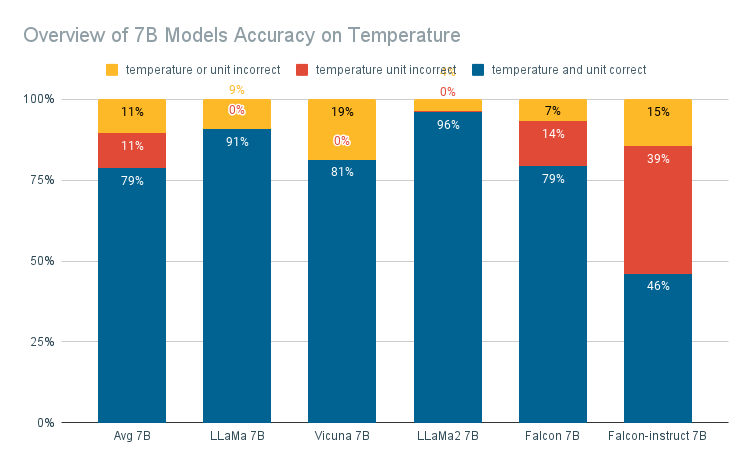
\includegraphics[height=0.7\textheight]{overview_7b_temp}
    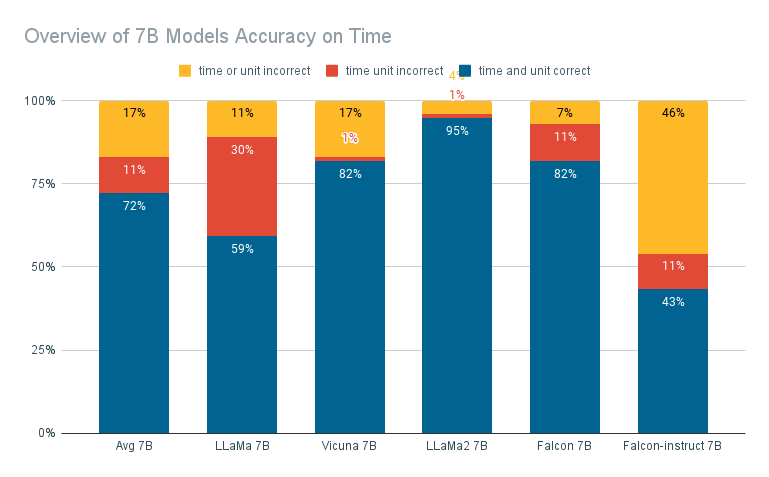
\includegraphics[height=0.7\textheight]{overview_7b_time}
    % \begin{columns}
    %     \column{0.35\textwidth}
    % 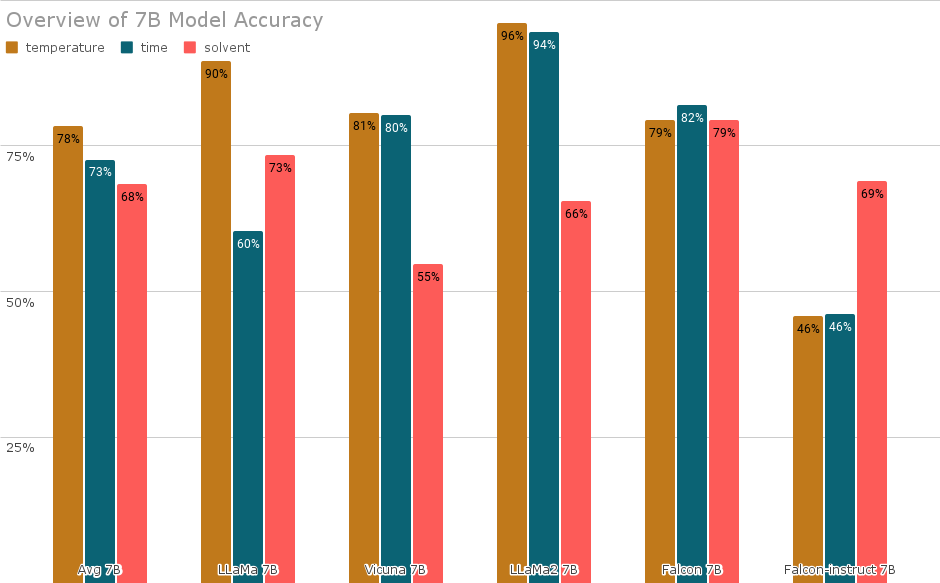
\includegraphics[width=\textwidth]{overview_7b_accuracy}
    % \column{0.65\textwidth}
    % 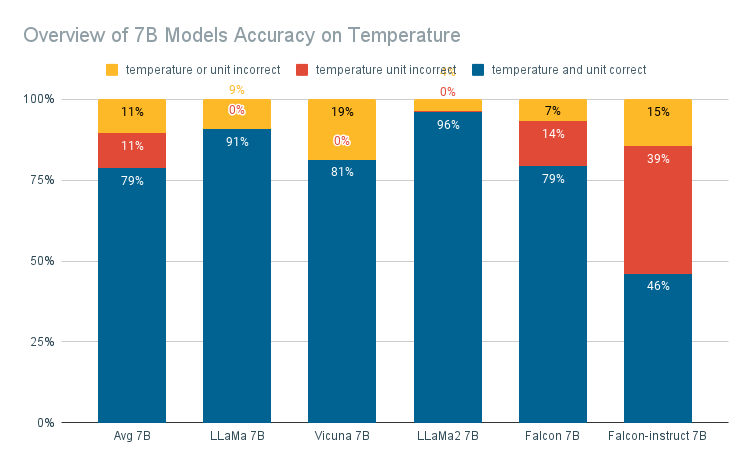
\includegraphics[height=0.7\textheight]{overview_7b_temp}
    % \end{columns}
    % \newpage
    % \begin{columns}
    %     \column{0.35\textwidth}
    % 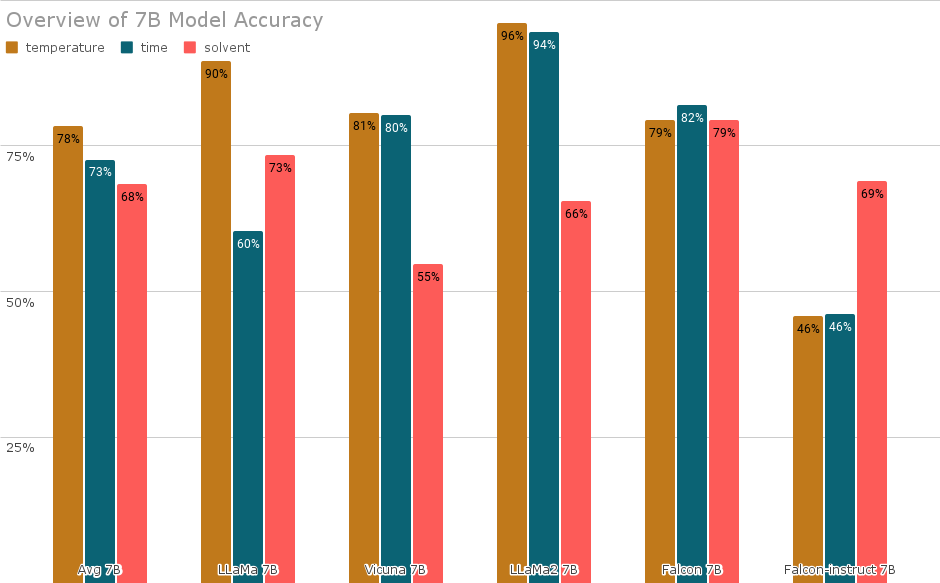
\includegraphics[width=\textwidth]{overview_7b_accuracy}
    % \column{0.65\textwidth}
    % 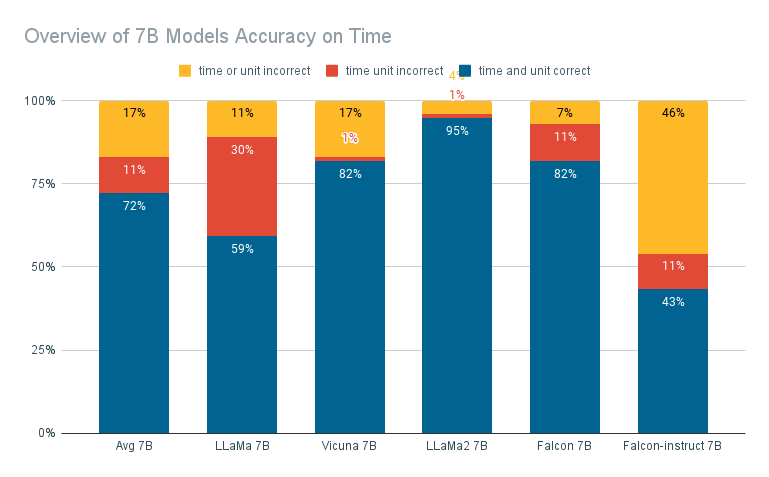
\includegraphics[height=0.7\textheight]{overview_7b_time}
    % \end{columns}
\end{frame}

\begin{frame}<handout>[c]{Note on Unit Confusion}
    \Large 
    \begin{itemize}
        \item Does happen fewer than 0.5\% (0-4 cases) for models sized 13B or more
    \end{itemize}
\end{frame}

\begin{frame}[c,fragile,allowframebreaks]{Solvent Resolution}
    \centering
    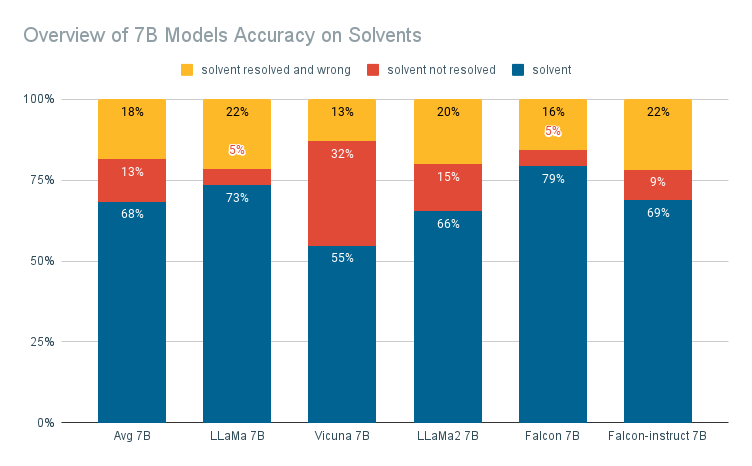
\includegraphics[height=0.7\textheight]{overview_7b_solv}
    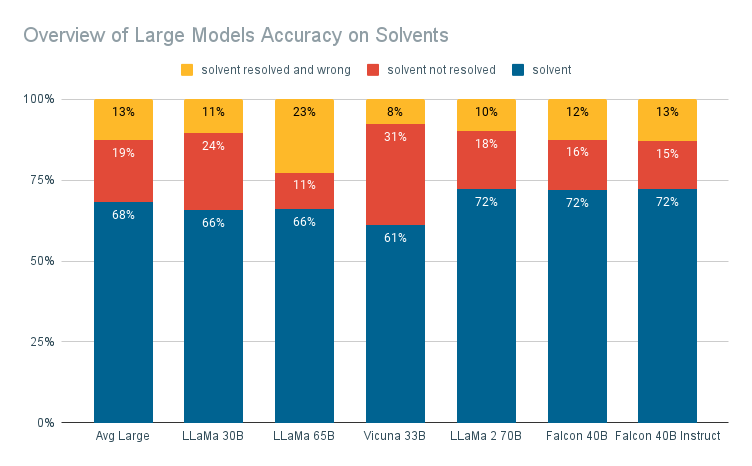
\includegraphics[height=0.7\textheight]{overview_large_solv}
\end{frame}


\begin{frame}[c]{Solvent Resolution?}
    \large
    One hypothesis: Models \textit{are} getting more accurate, but there is a failure in resolving the compounds.

    \vspace{2em}
    \pause

    Remember `distilled H2O'?

    \vspace{2em}
    \pause

    This may be true in particular for the \tsolv \texttt{N,N-DIMETHYLACETAMIDE} (\texttt{cid} 31374), where the synthesis paragraphs contain none of its 125 synonyms in 34 cases (or about 4.37\% of the dataset). 
\end{frame}

\begin{frame}[c]{Fine-Tuning: Excerpt 1}
    \code{input.py}{input}{Excerpt of what could be found in a custom dataloader. \mpy{text} describes any string the model may be provided as input. The tokenizer converts any string to a list of tokens and an attention mask, among other things.\\
    Similar code can be found in tutorials and official sources, e.g. \gls{microsoft} \cite{deepspeedexamples_2023}
}
\end{frame}


\begin{frame}[c]{Fine-Tuning: Failure 1}
    \code{output2.py}{output2}{A model fine-tuned like this returns the following. The \mpy{"} where actually inserted during conversion to \texttt{json} from \texttt{jsonformer}.}
    \only<handout>{
        \large
        Fundamentally, no idea what is going on. It works for others, and it could still be one of many different things that actuatlly happened.
    }
\end{frame}


\begin{frame}[c]{Fine-Tuning: Excerpt 2} 
    \large
    \begin{itemize}[<+(1)->]
        \item Using the \gls{hf} \texttt{trl} (Transformer Reinforcement Learning) library
        \item \mpy{DataCollator} are used for batch-processing inputs
        \item \mpy{DataCollatorForLanguageModeling} abstracting away tokenization, uses \mpy{"text"}-key for training in other examples
        \item Specifically, the example uses \mpy{DataCollatorForCompletionOnlyLM}, deriving from it
    \end{itemize}
\end{frame}


\begin{frame}[c]{Fine-Tuning: Failure 2}
    \code{error.py}{error}{Error when providing \mpy{DataCollatorForCompletionOnlyLM} with a dataloader similar to those in examples.\\Counterintuitively, this is not a \mpy{KeyError}.}
    It also fails when manually tokenizing before the \mpy{DataCollator} (providing tokenized \mpy{"input_ids"} etc. as key, using this or a different \mpy{DataCollator}).
\end{frame}

\chapter{Conclusion}\label{chap:conclusion}
\todo{write conclusion}
\todo{combine scientific question with results}

what was learned, in detail, from the experiments

\Appendix

\addchap{Appendix}

\todo{build automated json-to-tables/graphs for all raw values}

\todototoc
\listoftodos

\TheBibliography
\printbibliography[heading=bibintoc]

\end{document}
